\section{The Quantum Phase Transition}\label{ch:QuantumPhaseTransition}
One of the most interesting features of the Dicke model is its phase transition.
In the thermodynamic limit of infinite spin length or in the classic oscillator limit of vanishing oscillator frequency, there is a transition of the ground state to a parity breaking state at critical coupling $\gamma_c$.
This can easily be calculated in the classical limit, by minimizing the energy. 
It should be mentioned that the phase transition does not occur for finite spin length and finite oscillator frequency, because of the finite overlap of the two degenerate states, which allow a parity restoring superposition, with lowered energy \cite{LBAA12}.
That is why it has been argues by Larons and Irish that the phase transition is not quantum at all, but a purely classical phenomenon, basically just a bifurcation of the classical minimum energy state \cite{JLEKI17}.
There has been lots of research concerning the phase transition [?-?] and it has gained renewed interest recently, by its experimental realization in a Bose-Einstein-condensate by Baumann et al. \cite{KBCG+10}.
Since the phase transition itself relies on the parity to be conserved in the system (it is the symmetry that is spontaneously broken), the generalized system without conserved parity will not show a phase transition.
Nonetheless, since the $J_x$ term of he Hamiltonian can be interpreted as a symmetry breaking field, the system can be used to analyze the phase transition, if the additional field is small, i.e. $\sin\alpha \ll \cos \alpha$.
It is also worth mentioning that the choice of $\delta$, while changing the critical coupling $\gamma_c$ does not influence the nature of the phase transition, let alone whether it occurs or not.
Since most aspects of the phase transition have already been discussed, I will keep this chapter short, and only show the basics aspects of the phase transition.
Since the actual phase transition only occurs in the thermodynamic limit, finite spin length can only approximate the results.
Still it is notable that the ground state undergoes a significant change as the coupling constant rises.
For large and small coupling strengths compared to the critical value, there is almost perfect agreement with the classical model, if suitable measures are studied.

%Ground state phase transition
A phase transition generally is understood to be a rapid change in physical properties of a system as the value of a control parameter changes across a certain critical value.
As depicted in chapter \ref{ch:ClassLim}, the classical limit of the Dicke model displays such a fundamental change in its state of minimum energy as the coupling strength exceeds the critical value of $\gamma_c$ if the parity is conserved.
As the order parameter to describe the phase transition the coordinate $Q$ of the point or points of minimum energy is chosen.
For $\gamma \leq \gamma_c$ it is $Q = 0$, we will call this the normal phase, where the ground state of the spin boson model is a state of no excitations. 
If the coupling exceeds the critical value $\gamma > \gamma_c$ we find the nontrivial value of $Q = \pm \sqrt{\frac{2}{\nu}\left(\lambda - \frac{1}{4\lambda}\right)}$ with $\lambda$ as in equation \eqref{eq:lambdaCP}, if we chose $0 < \delta < \frac{\pi}{2}$. 
In order to study the quantum phase transition of the ground state a suitable way to compare the classical points of minimum energy to the quantum mechanical ground state is necessary.
Thus a projection that shows the oscillator part of the wave function is needed.
Any given state can be written in the basis of products of fock states and $J_z$-eigenstates with expansion coefficients $\beta_{n,m}$ so that it is 
\begin{equation}
	\ket{\Psi} = \sum\limits_{n=0}^{\infty}\sum\limits_{m=-j}^{j}\beta_{n,m}\ket{n}\ket{m} = \sum\limits_{n,m}\beta_{n,m}\ket{n,m}~~.
\end{equation}
The Husimi-oscillator projection $Q_\text{Osc}$ projects the oscillator part of the state onto a coherent state, while tracing out the spin part
\begin{equation}
	Q_ \text{Osc} (q,p)= \sum\limits_{m} |\braket{\alpha,m|\Psi}|^2 = \sum\limits_{m}|\sum\limits_{n}\beta_{n,m} \braket{\alpha(q,p)|n}|^2~~.
\end{equation}
Here $q$ and $p$ are the coordinates of the oscillator, which define the parameter of the coherent state via $\alpha = \sqrt{\frac{j}{2}} \left(q +i p\right)$ as described in chapter \ref{ch:CoherentStates}.
The projection of the ground state is shown in figure \ref{fig:groundstate} for different parameter choices.
\begin{figure}[h]
  \centering
  % GNUPLOT: LaTeX picture with Postscript
\begingroup
  \makeatletter
  \providecommand\color[2][]{%
    \GenericError{(gnuplot) \space\space\space\@spaces}{%
      Package color not loaded in conjunction with
      terminal option `colourtext'%
    }{See the gnuplot documentation for explanation.%
    }{Either use 'blacktext' in gnuplot or load the package
      color.sty in LaTeX.}%
    \renewcommand\color[2][]{}%
  }%
  \providecommand\includegraphics[2][]{%
    \GenericError{(gnuplot) \space\space\space\@spaces}{%
      Package graphicx or graphics not loaded%
    }{See the gnuplot documentation for explanation.%
    }{The gnuplot epslatex terminal needs graphicx.sty or graphics.sty.}%
    \renewcommand\includegraphics[2][]{}%
  }%
  \providecommand\rotatebox[2]{#2}%
  \@ifundefined{ifGPcolor}{%
    \newif\ifGPcolor
    \GPcolortrue
  }{}%
  \@ifundefined{ifGPblacktext}{%
    \newif\ifGPblacktext
    \GPblacktexttrue
  }{}%
  % define a \g@addto@macro without @ in the name:
  \let\gplgaddtomacro\g@addto@macro
  % define empty templates for all commands taking text:
  \gdef\gplbacktext{}%
  \gdef\gplfronttext{}%
  \makeatother
  \ifGPblacktext
    % no textcolor at all
    \def\colorrgb#1{}%
    \def\colorgray#1{}%
  \else
    % gray or color?
    \ifGPcolor
      \def\colorrgb#1{\color[rgb]{#1}}%
      \def\colorgray#1{\color[gray]{#1}}%
      \expandafter\def\csname LTw\endcsname{\color{white}}%
      \expandafter\def\csname LTb\endcsname{\color{black}}%
      \expandafter\def\csname LTa\endcsname{\color{black}}%
      \expandafter\def\csname LT0\endcsname{\color[rgb]{1,0,0}}%
      \expandafter\def\csname LT1\endcsname{\color[rgb]{0,1,0}}%
      \expandafter\def\csname LT2\endcsname{\color[rgb]{0,0,1}}%
      \expandafter\def\csname LT3\endcsname{\color[rgb]{1,0,1}}%
      \expandafter\def\csname LT4\endcsname{\color[rgb]{0,1,1}}%
      \expandafter\def\csname LT5\endcsname{\color[rgb]{1,1,0}}%
      \expandafter\def\csname LT6\endcsname{\color[rgb]{0,0,0}}%
      \expandafter\def\csname LT7\endcsname{\color[rgb]{1,0.3,0}}%
      \expandafter\def\csname LT8\endcsname{\color[rgb]{0.5,0.5,0.5}}%
    \else
      % gray
      \def\colorrgb#1{\color{black}}%
      \def\colorgray#1{\color[gray]{#1}}%
      \expandafter\def\csname LTw\endcsname{\color{white}}%
      \expandafter\def\csname LTb\endcsname{\color{black}}%
      \expandafter\def\csname LTa\endcsname{\color{black}}%
      \expandafter\def\csname LT0\endcsname{\color{black}}%
      \expandafter\def\csname LT1\endcsname{\color{black}}%
      \expandafter\def\csname LT2\endcsname{\color{black}}%
      \expandafter\def\csname LT3\endcsname{\color{black}}%
      \expandafter\def\csname LT4\endcsname{\color{black}}%
      \expandafter\def\csname LT5\endcsname{\color{black}}%
      \expandafter\def\csname LT6\endcsname{\color{black}}%
      \expandafter\def\csname LT7\endcsname{\color{black}}%
      \expandafter\def\csname LT8\endcsname{\color{black}}%
    \fi
  \fi
    \setlength{\unitlength}{0.0500bp}%
    \ifx\gptboxheight\undefined%
      \newlength{\gptboxheight}%
      \newlength{\gptboxwidth}%
      \newsavebox{\gptboxtext}%
    \fi%
    \setlength{\fboxrule}{0.5pt}%
    \setlength{\fboxsep}{1pt}%
\begin{picture}(6802.00,4534.00)%
    \gplgaddtomacro\gplbacktext{%
      \csname LTb\endcsname%
      \put(1133,4209){\makebox(0,0){\strut{}$\delta = 0, \alpha = 0$}}%
    }%
    \gplgaddtomacro\gplfronttext{%
      \csname LTb\endcsname%
      \put(364,2802){\makebox(0,0){\strut{}$-5$}}%
      \put(456,2781){\makebox(0,0){\strut{}$-4$}}%
      \put(547,2761){\makebox(0,0){\strut{}$-3$}}%
      \put(639,2741){\makebox(0,0){\strut{}$-2$}}%
      \put(731,2720){\makebox(0,0){\strut{}$-1$}}%
      \put(822,2700){\makebox(0,0){\strut{}$0$}}%
      \put(914,2679){\makebox(0,0){\strut{}$1$}}%
      \put(1005,2659){\makebox(0,0){\strut{}$2$}}%
      \put(1097,2639){\makebox(0,0){\strut{}$3$}}%
      \put(1188,2618){\makebox(0,0){\strut{}$4$}}%
      \put(1279,2598){\makebox(0,0){\strut{}$5$}}%
      \put(737,2664){\makebox(0,0){\strut{}$q$}}%
      \put(1388,2627){\makebox(0,0){\strut{}$-5$}}%
      \put(1441,2662){\makebox(0,0){\strut{}$-4$}}%
      \put(1494,2697){\makebox(0,0){\strut{}$-3$}}%
      \put(1547,2733){\makebox(0,0){\strut{}$-2$}}%
      \put(1600,2768){\makebox(0,0){\strut{}$-1$}}%
      \put(1653,2803){\makebox(0,0){\strut{}$0$}}%
      \put(1706,2838){\makebox(0,0){\strut{}$1$}}%
      \put(1759,2874){\makebox(0,0){\strut{}$2$}}%
      \put(1812,2909){\makebox(0,0){\strut{}$3$}}%
      \put(1865,2944){\makebox(0,0){\strut{}$4$}}%
      \put(1917,2979){\makebox(0,0){\strut{}$5$}}%
      \put(1820,2775){\makebox(0,0){\strut{}$p$}}%
      \put(285,3089){\makebox(0,0)[r]{\strut{}$10^{-20}$}}%
      \put(285,3206){\makebox(0,0)[r]{\strut{}$10^{-15}$}}%
      \put(285,3323){\makebox(0,0)[r]{\strut{}$10^{-10}$}}%
      \put(285,3440){\makebox(0,0)[r]{\strut{}$10^{-5}$}}%
      \put(285,3557){\makebox(0,0)[r]{\strut{}$10^{0}$}}%
    }%
    \gplgaddtomacro\gplbacktext{%
      \csname LTb\endcsname%
      \put(3400,4161){\makebox(0,0){\strut{}$\delta = \pi /4, \alpha = 0$}}%
    }%
    \gplgaddtomacro\gplfronttext{%
      \csname LTb\endcsname%
      \put(2627,2778){\makebox(0,0){\strut{}$-5$}}%
      \put(2718,2759){\makebox(0,0){\strut{}$-4$}}%
      \put(2810,2741){\makebox(0,0){\strut{}$-3$}}%
      \put(2902,2722){\makebox(0,0){\strut{}$-2$}}%
      \put(2993,2703){\makebox(0,0){\strut{}$-1$}}%
      \put(3085,2685){\makebox(0,0){\strut{}$0$}}%
      \put(3177,2666){\makebox(0,0){\strut{}$1$}}%
      \put(3268,2647){\makebox(0,0){\strut{}$2$}}%
      \put(3360,2629){\makebox(0,0){\strut{}$3$}}%
      \put(3450,2610){\makebox(0,0){\strut{}$4$}}%
      \put(3542,2592){\makebox(0,0){\strut{}$5$}}%
      \put(3004,2656){\makebox(0,0){\strut{}$q$}}%
      \put(3655,2622){\makebox(0,0){\strut{}$-5$}}%
      \put(3708,2655){\makebox(0,0){\strut{}$-4$}}%
      \put(3761,2687){\makebox(0,0){\strut{}$-3$}}%
      \put(3814,2719){\makebox(0,0){\strut{}$-2$}}%
      \put(3867,2751){\makebox(0,0){\strut{}$-1$}}%
      \put(3920,2784){\makebox(0,0){\strut{}$0$}}%
      \put(3973,2816){\makebox(0,0){\strut{}$1$}}%
      \put(4026,2848){\makebox(0,0){\strut{}$2$}}%
      \put(4079,2880){\makebox(0,0){\strut{}$3$}}%
      \put(4132,2913){\makebox(0,0){\strut{}$4$}}%
      \put(4184,2945){\makebox(0,0){\strut{}$5$}}%
      \put(4087,2758){\makebox(0,0){\strut{}$p$}}%
      \put(2552,3045){\makebox(0,0)[r]{\strut{}$10^{-20}$}}%
      \put(2552,3152){\makebox(0,0)[r]{\strut{}$10^{-15}$}}%
      \put(2552,3259){\makebox(0,0)[r]{\strut{}$10^{-10}$}}%
      \put(2552,3366){\makebox(0,0)[r]{\strut{}$10^{-5}$}}%
      \put(2552,3474){\makebox(0,0)[r]{\strut{}$10^{0}$}}%
    }%
    \gplgaddtomacro\gplbacktext{%
      \csname LTb\endcsname%
      \put(5667,4161){\makebox(0,0){\strut{}$\delta = \pi /2, \alpha = 0$}}%
    }%
    \gplgaddtomacro\gplfronttext{%
      \csname LTb\endcsname%
      \put(4894,2778){\makebox(0,0){\strut{}$-5$}}%
      \put(4985,2759){\makebox(0,0){\strut{}$-4$}}%
      \put(5077,2741){\makebox(0,0){\strut{}$-3$}}%
      \put(5169,2722){\makebox(0,0){\strut{}$-2$}}%
      \put(5260,2703){\makebox(0,0){\strut{}$-1$}}%
      \put(5352,2685){\makebox(0,0){\strut{}$0$}}%
      \put(5444,2666){\makebox(0,0){\strut{}$1$}}%
      \put(5535,2647){\makebox(0,0){\strut{}$2$}}%
      \put(5627,2629){\makebox(0,0){\strut{}$3$}}%
      \put(5717,2610){\makebox(0,0){\strut{}$4$}}%
      \put(5809,2592){\makebox(0,0){\strut{}$5$}}%
      \put(5271,2656){\makebox(0,0){\strut{}$q$}}%
      \put(5922,2622){\makebox(0,0){\strut{}$-5$}}%
      \put(5975,2655){\makebox(0,0){\strut{}$-4$}}%
      \put(6028,2687){\makebox(0,0){\strut{}$-3$}}%
      \put(6081,2719){\makebox(0,0){\strut{}$-2$}}%
      \put(6134,2751){\makebox(0,0){\strut{}$-1$}}%
      \put(6187,2784){\makebox(0,0){\strut{}$0$}}%
      \put(6240,2816){\makebox(0,0){\strut{}$1$}}%
      \put(6293,2848){\makebox(0,0){\strut{}$2$}}%
      \put(6346,2880){\makebox(0,0){\strut{}$3$}}%
      \put(6399,2913){\makebox(0,0){\strut{}$4$}}%
      \put(6451,2945){\makebox(0,0){\strut{}$5$}}%
      \put(6354,2758){\makebox(0,0){\strut{}$p$}}%
      \put(4819,3045){\makebox(0,0)[r]{\strut{}$10^{-20}$}}%
      \put(4819,3152){\makebox(0,0)[r]{\strut{}$10^{-15}$}}%
      \put(4819,3259){\makebox(0,0)[r]{\strut{}$10^{-10}$}}%
      \put(4819,3366){\makebox(0,0)[r]{\strut{}$10^{-5}$}}%
      \put(4819,3474){\makebox(0,0)[r]{\strut{}$10^{0}$}}%
    }%
    \gplgaddtomacro\gplbacktext{%
      \csname LTb\endcsname%
      \put(1133,1894){\makebox(0,0){\strut{}$\delta = 3\pi /4, \alpha = 0$}}%
    }%
    \gplgaddtomacro\gplfronttext{%
      \csname LTb\endcsname%
      \put(360,511){\makebox(0,0){\strut{}$-5$}}%
      \put(451,492){\makebox(0,0){\strut{}$-4$}}%
      \put(543,474){\makebox(0,0){\strut{}$-3$}}%
      \put(635,455){\makebox(0,0){\strut{}$-2$}}%
      \put(726,436){\makebox(0,0){\strut{}$-1$}}%
      \put(818,418){\makebox(0,0){\strut{}$0$}}%
      \put(910,399){\makebox(0,0){\strut{}$1$}}%
      \put(1001,380){\makebox(0,0){\strut{}$2$}}%
      \put(1093,362){\makebox(0,0){\strut{}$3$}}%
      \put(1183,343){\makebox(0,0){\strut{}$4$}}%
      \put(1275,325){\makebox(0,0){\strut{}$5$}}%
      \put(737,389){\makebox(0,0){\strut{}$q$}}%
      \put(1388,355){\makebox(0,0){\strut{}$-5$}}%
      \put(1441,388){\makebox(0,0){\strut{}$-4$}}%
      \put(1494,420){\makebox(0,0){\strut{}$-3$}}%
      \put(1547,452){\makebox(0,0){\strut{}$-2$}}%
      \put(1600,484){\makebox(0,0){\strut{}$-1$}}%
      \put(1653,517){\makebox(0,0){\strut{}$0$}}%
      \put(1706,549){\makebox(0,0){\strut{}$1$}}%
      \put(1759,581){\makebox(0,0){\strut{}$2$}}%
      \put(1812,613){\makebox(0,0){\strut{}$3$}}%
      \put(1865,646){\makebox(0,0){\strut{}$4$}}%
      \put(1917,678){\makebox(0,0){\strut{}$5$}}%
      \put(1820,491){\makebox(0,0){\strut{}$p$}}%
      \put(285,778){\makebox(0,0)[r]{\strut{}$10^{-20}$}}%
      \put(285,885){\makebox(0,0)[r]{\strut{}$10^{-15}$}}%
      \put(285,992){\makebox(0,0)[r]{\strut{}$10^{-10}$}}%
      \put(285,1099){\makebox(0,0)[r]{\strut{}$10^{-5}$}}%
      \put(285,1207){\makebox(0,0)[r]{\strut{}$10^{0}$}}%
    }%
    \gplgaddtomacro\gplbacktext{%
      \csname LTb\endcsname%
      \put(3400,1846){\makebox(0,0){\strut{}$\delta = \pi /4, \alpha = \pi /100$}}%
    }%
    \gplgaddtomacro\gplfronttext{%
      \csname LTb\endcsname%
      \put(2622,486){\makebox(0,0){\strut{}$-5$}}%
      \put(2713,470){\makebox(0,0){\strut{}$-4$}}%
      \put(2805,453){\makebox(0,0){\strut{}$-3$}}%
      \put(2896,436){\makebox(0,0){\strut{}$-2$}}%
      \put(2988,419){\makebox(0,0){\strut{}$-1$}}%
      \put(3080,402){\makebox(0,0){\strut{}$0$}}%
      \put(3171,385){\makebox(0,0){\strut{}$1$}}%
      \put(3263,368){\makebox(0,0){\strut{}$2$}}%
      \put(3355,351){\makebox(0,0){\strut{}$3$}}%
      \put(3445,334){\makebox(0,0){\strut{}$4$}}%
      \put(3537,317){\makebox(0,0){\strut{}$5$}}%
      \put(3004,380){\makebox(0,0){\strut{}$q$}}%
      \put(3655,350){\makebox(0,0){\strut{}$-5$}}%
      \put(3708,379){\makebox(0,0){\strut{}$-4$}}%
      \put(3761,409){\makebox(0,0){\strut{}$-3$}}%
      \put(3814,438){\makebox(0,0){\strut{}$-2$}}%
      \put(3867,467){\makebox(0,0){\strut{}$-1$}}%
      \put(3920,497){\makebox(0,0){\strut{}$0$}}%
      \put(3973,526){\makebox(0,0){\strut{}$1$}}%
      \put(4026,555){\makebox(0,0){\strut{}$2$}}%
      \put(4079,584){\makebox(0,0){\strut{}$3$}}%
      \put(4132,614){\makebox(0,0){\strut{}$4$}}%
      \put(4184,643){\makebox(0,0){\strut{}$5$}}%
      \put(4087,473){\makebox(0,0){\strut{}$p$}}%
      \put(2552,734){\makebox(0,0)[r]{\strut{}$10^{-20}$}}%
      \put(2552,832){\makebox(0,0)[r]{\strut{}$10^{-15}$}}%
      \put(2552,928){\makebox(0,0)[r]{\strut{}$10^{-10}$}}%
      \put(2552,1026){\makebox(0,0)[r]{\strut{}$10^{-5}$}}%
      \put(2552,1124){\makebox(0,0)[r]{\strut{}$10^{0}$}}%
    }%
    \gplgaddtomacro\gplbacktext{%
      \csname LTb\endcsname%
      \put(5667,1846){\makebox(0,0){\strut{}$\delta = \pi /4, \alpha = -\pi /100$}}%
    }%
    \gplgaddtomacro\gplfronttext{%
      \csname LTb\endcsname%
      \put(4889,486){\makebox(0,0){\strut{}$-5$}}%
      \put(4980,470){\makebox(0,0){\strut{}$-4$}}%
      \put(5072,453){\makebox(0,0){\strut{}$-3$}}%
      \put(5163,436){\makebox(0,0){\strut{}$-2$}}%
      \put(5255,419){\makebox(0,0){\strut{}$-1$}}%
      \put(5347,402){\makebox(0,0){\strut{}$0$}}%
      \put(5438,385){\makebox(0,0){\strut{}$1$}}%
      \put(5530,368){\makebox(0,0){\strut{}$2$}}%
      \put(5622,351){\makebox(0,0){\strut{}$3$}}%
      \put(5712,334){\makebox(0,0){\strut{}$4$}}%
      \put(5804,317){\makebox(0,0){\strut{}$5$}}%
      \put(5271,380){\makebox(0,0){\strut{}$q$}}%
      \put(5922,350){\makebox(0,0){\strut{}$-5$}}%
      \put(5975,379){\makebox(0,0){\strut{}$-4$}}%
      \put(6028,409){\makebox(0,0){\strut{}$-3$}}%
      \put(6081,438){\makebox(0,0){\strut{}$-2$}}%
      \put(6134,467){\makebox(0,0){\strut{}$-1$}}%
      \put(6187,497){\makebox(0,0){\strut{}$0$}}%
      \put(6240,526){\makebox(0,0){\strut{}$1$}}%
      \put(6293,555){\makebox(0,0){\strut{}$2$}}%
      \put(6346,584){\makebox(0,0){\strut{}$3$}}%
      \put(6399,614){\makebox(0,0){\strut{}$4$}}%
      \put(6451,643){\makebox(0,0){\strut{}$5$}}%
      \put(6354,473){\makebox(0,0){\strut{}$p$}}%
      \put(4819,734){\makebox(0,0)[r]{\strut{}$10^{-20}$}}%
      \put(4819,832){\makebox(0,0)[r]{\strut{}$10^{-15}$}}%
      \put(4819,928){\makebox(0,0)[r]{\strut{}$10^{-10}$}}%
      \put(4819,1026){\makebox(0,0)[r]{\strut{}$10^{-5}$}}%
      \put(4819,1124){\makebox(0,0)[r]{\strut{}$10^{0}$}}%
    }%
    \gplbacktext
    \put(0,0){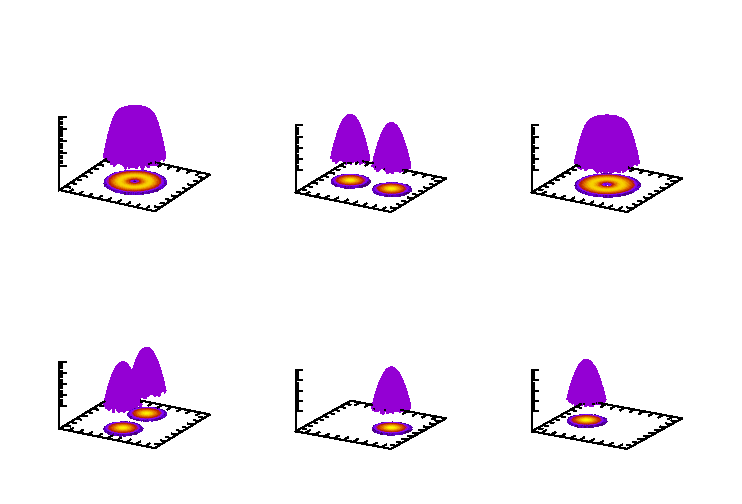
\includegraphics{figures/tex/groundstate}}%
    \gplfronttext
  \end{picture}%
\endgroup

  \caption{groundstate for $j= 30, \gamma = 2, \nu = 0.8, \delta$ and $\alpha$ as given \\ \textcolor{red}{adjust the plot}}\label{fig:groundstate}
\end{figure}
As expected, they resemble the classical ground state, by displaying a high value the points of $Q$ and $P$ of the classical minimum energy state. 
For large spin the ground state will resemble a product state of coherent states in both oscillator and spin part, so it is reasonable to assume a gaussian distribution around the points of the classical ground state.
Thus, gaussian curves can be fitted through the projection of the ground state along the $p = 0$ axis. 
The choice of this axis is of course due to the fact $P=0$ in the classical ground state.
The fitting function takes the form of
\begin{equation}
 Q_\text{fit} = N\left( e^{ - \frac{(q - \mu)^2}{\sigma^2}} + \delta_{\alpha,0} e^{ - \frac{(q + \mu)^2}{\sigma^2}}  \right)~~,         
\label{eq:fit}
\end{equation}
where $\delta_{\alpha,0}$ is zero unless parity is conserved, which respect the loss of symmetry if parity is broken.
The parameter $\mu$ can be considered to be a shift of the grounstate away from the position at $q = 0$, moreso if the parity is broken, since then only one peak is present.
The parameter $\sigma$ describes the width of the gaussian and will ideally remain constant in absolute values, or fall as $1/\sqrt{j}$ in the rescaled values for $q$.

%results
%general ground state discussion
Surprisingly this fit matches almost perfectly even for small spins and for arbitrary coupling strength, exhibiting the biggest deviations for coupling strengths close to the critical coupling.
%energy discussion


%mu discussion for different j parity conserved


%mu discussion for different \alpha
\begin{figure}[h]
  \centering
  % GNUPLOT: LaTeX picture with Postscript
\begingroup
  \makeatletter
  \providecommand\color[2][]{%
    \GenericError{(gnuplot) \space\space\space\@spaces}{%
      Package color not loaded in conjunction with
      terminal option `colourtext'%
    }{See the gnuplot documentation for explanation.%
    }{Either use 'blacktext' in gnuplot or load the package
      color.sty in LaTeX.}%
    \renewcommand\color[2][]{}%
  }%
  \providecommand\includegraphics[2][]{%
    \GenericError{(gnuplot) \space\space\space\@spaces}{%
      Package graphicx or graphics not loaded%
    }{See the gnuplot documentation for explanation.%
    }{The gnuplot epslatex terminal needs graphicx.sty or graphics.sty.}%
    \renewcommand\includegraphics[2][]{}%
  }%
  \providecommand\rotatebox[2]{#2}%
  \@ifundefined{ifGPcolor}{%
    \newif\ifGPcolor
    \GPcolortrue
  }{}%
  \@ifundefined{ifGPblacktext}{%
    \newif\ifGPblacktext
    \GPblacktexttrue
  }{}%
  % define a \g@addto@macro without @ in the name:
  \let\gplgaddtomacro\g@addto@macro
  % define empty templates for all commands taking text:
  \gdef\gplbacktext{}%
  \gdef\gplfronttext{}%
  \makeatother
  \ifGPblacktext
    % no textcolor at all
    \def\colorrgb#1{}%
    \def\colorgray#1{}%
  \else
    % gray or color?
    \ifGPcolor
      \def\colorrgb#1{\color[rgb]{#1}}%
      \def\colorgray#1{\color[gray]{#1}}%
      \expandafter\def\csname LTw\endcsname{\color{white}}%
      \expandafter\def\csname LTb\endcsname{\color{black}}%
      \expandafter\def\csname LTa\endcsname{\color{black}}%
      \expandafter\def\csname LT0\endcsname{\color[rgb]{1,0,0}}%
      \expandafter\def\csname LT1\endcsname{\color[rgb]{0,1,0}}%
      \expandafter\def\csname LT2\endcsname{\color[rgb]{0,0,1}}%
      \expandafter\def\csname LT3\endcsname{\color[rgb]{1,0,1}}%
      \expandafter\def\csname LT4\endcsname{\color[rgb]{0,1,1}}%
      \expandafter\def\csname LT5\endcsname{\color[rgb]{1,1,0}}%
      \expandafter\def\csname LT6\endcsname{\color[rgb]{0,0,0}}%
      \expandafter\def\csname LT7\endcsname{\color[rgb]{1,0.3,0}}%
      \expandafter\def\csname LT8\endcsname{\color[rgb]{0.5,0.5,0.5}}%
    \else
      % gray
      \def\colorrgb#1{\color{black}}%
      \def\colorgray#1{\color[gray]{#1}}%
      \expandafter\def\csname LTw\endcsname{\color{white}}%
      \expandafter\def\csname LTb\endcsname{\color{black}}%
      \expandafter\def\csname LTa\endcsname{\color{black}}%
      \expandafter\def\csname LT0\endcsname{\color{black}}%
      \expandafter\def\csname LT1\endcsname{\color{black}}%
      \expandafter\def\csname LT2\endcsname{\color{black}}%
      \expandafter\def\csname LT3\endcsname{\color{black}}%
      \expandafter\def\csname LT4\endcsname{\color{black}}%
      \expandafter\def\csname LT5\endcsname{\color{black}}%
      \expandafter\def\csname LT6\endcsname{\color{black}}%
      \expandafter\def\csname LT7\endcsname{\color{black}}%
      \expandafter\def\csname LT8\endcsname{\color{black}}%
    \fi
  \fi
    \setlength{\unitlength}{0.0500bp}%
    \ifx\gptboxheight\undefined%
      \newlength{\gptboxheight}%
      \newlength{\gptboxwidth}%
      \newsavebox{\gptboxtext}%
    \fi%
    \setlength{\fboxrule}{0.5pt}%
    \setlength{\fboxsep}{1pt}%
\begin{picture}(6802.00,4534.00)%
    \gplgaddtomacro\gplbacktext{%
      \csname LTb\endcsname%
      \put(814,704){\makebox(0,0)[r]{\strut{}$0$}}%
      \put(814,1417){\makebox(0,0)[r]{\strut{}$0.5$}}%
      \put(814,2130){\makebox(0,0)[r]{\strut{}$1$}}%
      \put(814,2843){\makebox(0,0)[r]{\strut{}$1.5$}}%
      \put(814,3556){\makebox(0,0)[r]{\strut{}$2$}}%
      \put(814,4269){\makebox(0,0)[r]{\strut{}$2.5$}}%
      \put(946,484){\makebox(0,0){\strut{}$0$}}%
      \put(1492,484){\makebox(0,0){\strut{}$0.2$}}%
      \put(2038,484){\makebox(0,0){\strut{}$0.4$}}%
      \put(2584,484){\makebox(0,0){\strut{}$0.6$}}%
      \put(3130,484){\makebox(0,0){\strut{}$0.8$}}%
      \put(3676,484){\makebox(0,0){\strut{}$1$}}%
      \put(4221,484){\makebox(0,0){\strut{}$1.2$}}%
      \put(4767,484){\makebox(0,0){\strut{}$1.4$}}%
      \put(5313,484){\makebox(0,0){\strut{}$1.6$}}%
      \put(5859,484){\makebox(0,0){\strut{}$1.8$}}%
      \put(6405,484){\makebox(0,0){\strut{}$2$}}%
    }%
    \gplgaddtomacro\gplfronttext{%
      \csname LTb\endcsname%
      \put(176,2486){\rotatebox{-270}{\makebox(0,0){\strut{}$\gamma$}}}%
      \put(3675,154){\makebox(0,0){\strut{}$\mu$}}%
      \csname LTb\endcsname%
      \put(2398,4096){\makebox(0,0)[r]{\strut{}$\alpha = 0$}}%
      \csname LTb\endcsname%
      \put(2398,3876){\makebox(0,0)[r]{\strut{}$\alpha = 0.001\pi$}}%
      \csname LTb\endcsname%
      \put(2398,3656){\makebox(0,0)[r]{\strut{}$\alpha = 0.01 \pi$}}%
      \csname LTb\endcsname%
      \put(2398,3436){\makebox(0,0)[r]{\strut{}$\alpha = 0.1 \pi$}}%
      \csname LTb\endcsname%
      \put(2398,3216){\makebox(0,0)[r]{\strut{}$\alpha = 0.5 \pi$}}%
    }%
    \gplbacktext
    \put(0,0){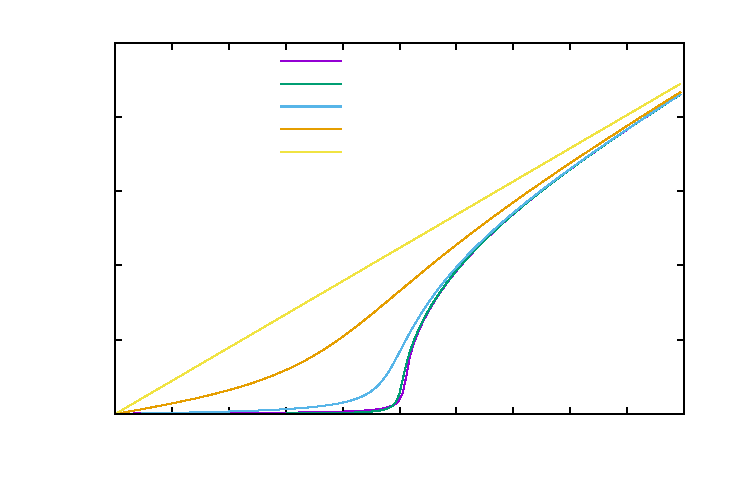
\includegraphics{figures/tex/phasetransition_alpha}}%
    \gplfronttext
  \end{picture}%
\endgroup

  \caption{groundstate shift $\mu$ for $\delta = \pi/4, \nu = 0.8$ for different values of $\alpha$ for $j = 100$ \textcolor{red}{adjust the plot?}}\label{fig:mu(gamma,alpha)}
\end{figure}
For small values of $\alpha$ the shift of the groundstate $\mu$ approaches the value for $\alpha = 0$, while for $\alpha = \pi/2$ a linear relation can be observed, which can be seen in the exact solvability of this system for any spin.
For $\delta = \pi/4$ and $\alpha = pi/2$ the Hamiltonian reads
\begin{equation}
  H = \nu a^\dagger a + J_x + \gamma (a + a^\dagger)J_x.
\end{equation}
The eigenstates are then product states of $J_x$ eigenstates and oscillator eingenstates shifted by $\sqrt{\frac{1}{\nu}\gamma m}$ where $m$ is the quantum number of the $J_x$ eigenstate.
\textcolor{red}{Should it not be $\sqrt{\gamma}$ then?}
%sigma discussion
\begin{figure}[h]
  \centering
  % GNUPLOT: LaTeX picture with Postscript
\begingroup
  \makeatletter
  \providecommand\color[2][]{%
    \GenericError{(gnuplot) \space\space\space\@spaces}{%
      Package color not loaded in conjunction with
      terminal option `colourtext'%
    }{See the gnuplot documentation for explanation.%
    }{Either use 'blacktext' in gnuplot or load the package
      color.sty in LaTeX.}%
    \renewcommand\color[2][]{}%
  }%
  \providecommand\includegraphics[2][]{%
    \GenericError{(gnuplot) \space\space\space\@spaces}{%
      Package graphicx or graphics not loaded%
    }{See the gnuplot documentation for explanation.%
    }{The gnuplot epslatex terminal needs graphicx.sty or graphics.sty.}%
    \renewcommand\includegraphics[2][]{}%
  }%
  \providecommand\rotatebox[2]{#2}%
  \@ifundefined{ifGPcolor}{%
    \newif\ifGPcolor
    \GPcolortrue
  }{}%
  \@ifundefined{ifGPblacktext}{%
    \newif\ifGPblacktext
    \GPblacktexttrue
  }{}%
  % define a \g@addto@macro without @ in the name:
  \let\gplgaddtomacro\g@addto@macro
  % define empty templates for all commands taking text:
  \gdef\gplbacktext{}%
  \gdef\gplfronttext{}%
  \makeatother
  \ifGPblacktext
    % no textcolor at all
    \def\colorrgb#1{}%
    \def\colorgray#1{}%
  \else
    % gray or color?
    \ifGPcolor
      \def\colorrgb#1{\color[rgb]{#1}}%
      \def\colorgray#1{\color[gray]{#1}}%
      \expandafter\def\csname LTw\endcsname{\color{white}}%
      \expandafter\def\csname LTb\endcsname{\color{black}}%
      \expandafter\def\csname LTa\endcsname{\color{black}}%
      \expandafter\def\csname LT0\endcsname{\color[rgb]{1,0,0}}%
      \expandafter\def\csname LT1\endcsname{\color[rgb]{0,1,0}}%
      \expandafter\def\csname LT2\endcsname{\color[rgb]{0,0,1}}%
      \expandafter\def\csname LT3\endcsname{\color[rgb]{1,0,1}}%
      \expandafter\def\csname LT4\endcsname{\color[rgb]{0,1,1}}%
      \expandafter\def\csname LT5\endcsname{\color[rgb]{1,1,0}}%
      \expandafter\def\csname LT6\endcsname{\color[rgb]{0,0,0}}%
      \expandafter\def\csname LT7\endcsname{\color[rgb]{1,0.3,0}}%
      \expandafter\def\csname LT8\endcsname{\color[rgb]{0.5,0.5,0.5}}%
    \else
      % gray
      \def\colorrgb#1{\color{black}}%
      \def\colorgray#1{\color[gray]{#1}}%
      \expandafter\def\csname LTw\endcsname{\color{white}}%
      \expandafter\def\csname LTb\endcsname{\color{black}}%
      \expandafter\def\csname LTa\endcsname{\color{black}}%
      \expandafter\def\csname LT0\endcsname{\color{black}}%
      \expandafter\def\csname LT1\endcsname{\color{black}}%
      \expandafter\def\csname LT2\endcsname{\color{black}}%
      \expandafter\def\csname LT3\endcsname{\color{black}}%
      \expandafter\def\csname LT4\endcsname{\color{black}}%
      \expandafter\def\csname LT5\endcsname{\color{black}}%
      \expandafter\def\csname LT6\endcsname{\color{black}}%
      \expandafter\def\csname LT7\endcsname{\color{black}}%
      \expandafter\def\csname LT8\endcsname{\color{black}}%
    \fi
  \fi
    \setlength{\unitlength}{0.0500bp}%
    \ifx\gptboxheight\undefined%
      \newlength{\gptboxheight}%
      \newlength{\gptboxwidth}%
      \newsavebox{\gptboxtext}%
    \fi%
    \setlength{\fboxrule}{0.5pt}%
    \setlength{\fboxsep}{1pt}%
\begin{picture}(4534.00,3400.00)%
    \gplgaddtomacro\gplbacktext{%
      \csname LTb\endcsname%
      \put(946,704){\makebox(0,0)[r]{\strut{}$0.01$}}%
      \put(946,1514){\makebox(0,0)[r]{\strut{}$0.1$}}%
      \put(946,2325){\makebox(0,0)[r]{\strut{}$1$}}%
      \put(946,3135){\makebox(0,0)[r]{\strut{}$10$}}%
      \put(1550,484){\makebox(0,0){\strut{}$1$}}%
      \put(2334,484){\makebox(0,0){\strut{}$10$}}%
      \put(3117,484){\makebox(0,0){\strut{}$100$}}%
      \put(3901,484){\makebox(0,0){\strut{}$1000$}}%
    }%
    \gplgaddtomacro\gplfronttext{%
      \csname LTb\endcsname%
      \put(176,1919){\rotatebox{-270}{\makebox(0,0){\strut{}$\sigma$}}}%
      \put(2607,154){\makebox(0,0){\strut{}$j$}}%
    }%
    \gplbacktext
    \put(0,0){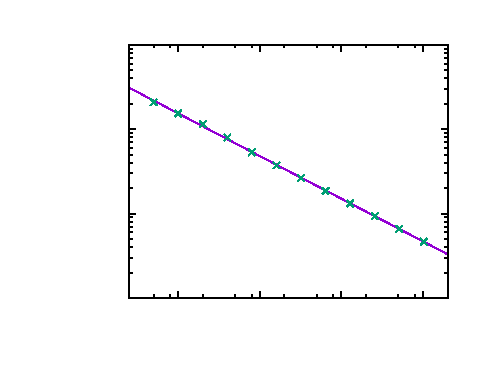
\includegraphics{figures/tex/sigma_j}}%
    \gplfronttext
  \end{picture}%
\endgroup

  \caption{Oscillator width $\sigma$ for different spin length and a linear fit \\
\textcolor{red}{adjust the plot, add more parameter sets}}\label{fig:sigma(j)}
\end{figure}
The fitting parameter $\sigma$ in equation \eqref{eq:fit} resembles the width of the gaussian curve.
It is shown in figure \ref{fig:sigma(j)} for different sets of parameters, and displays a proportionality of roughly $\sigma \propto 1/\sqrt{j}$, which can be understood by considering that the absolute value of the width of a coherent state is constant and that $q$ is rescaled by $\frac{1}{\sqrt{j}}$ (cf. equation \eqref{eq:variables}).
The logarithmic values for $\sigma$ for different $j$ are fitted by a linear function $\ln(\sigma) = a \ln(j) + b$ which appears linear in the double logarithmic scale. 
The fitting parameters are given in table \ref{tab:fitsigma}.
\begin{center}
 \begin{tabular}{|c|c|c|c|c|c|}
 \hline
  $\delta$ & $\alpha$ & $\gamma$ & $\nu$ & $a$ & $b$\\
\hline
  $\frac{\pi}{4}$ & $0$ & $1.3$ & $0.8$ & $-0.505\pm 0.003$ & $0.43\pm 0.01$\\
  \hline
\end{tabular}
\captionof{table}{Fitting parameters for $\sigma$ as a funtion of $j$ for different parameter sets}\label{tab:fitsigma}
\end{center}
\textcolor{red}{A sentence about different parameters.}

